\section{Zadanie 5} 
Pora wyznaczyć regulator dla naszego niestabilnego obiektu. Użyjemy struktury drugiego modelu w przestrzeni stanu. Ogólna struktura regulatora to:
\[
 u(k)=-KX(k)
\]

Wektor $K$ obliczamy poleceniem \mintinline{matlab}{Kd = acker(Ad,Bd,[z1 z2 z3])}, gdzie za \mintinline{matlab}{z1}, \mintinline{matlab}{z2} i \mintinline{matlab}{z3} ustalamy bieguny układu zamkniętego.
\begin{figure}[H]
\centering
 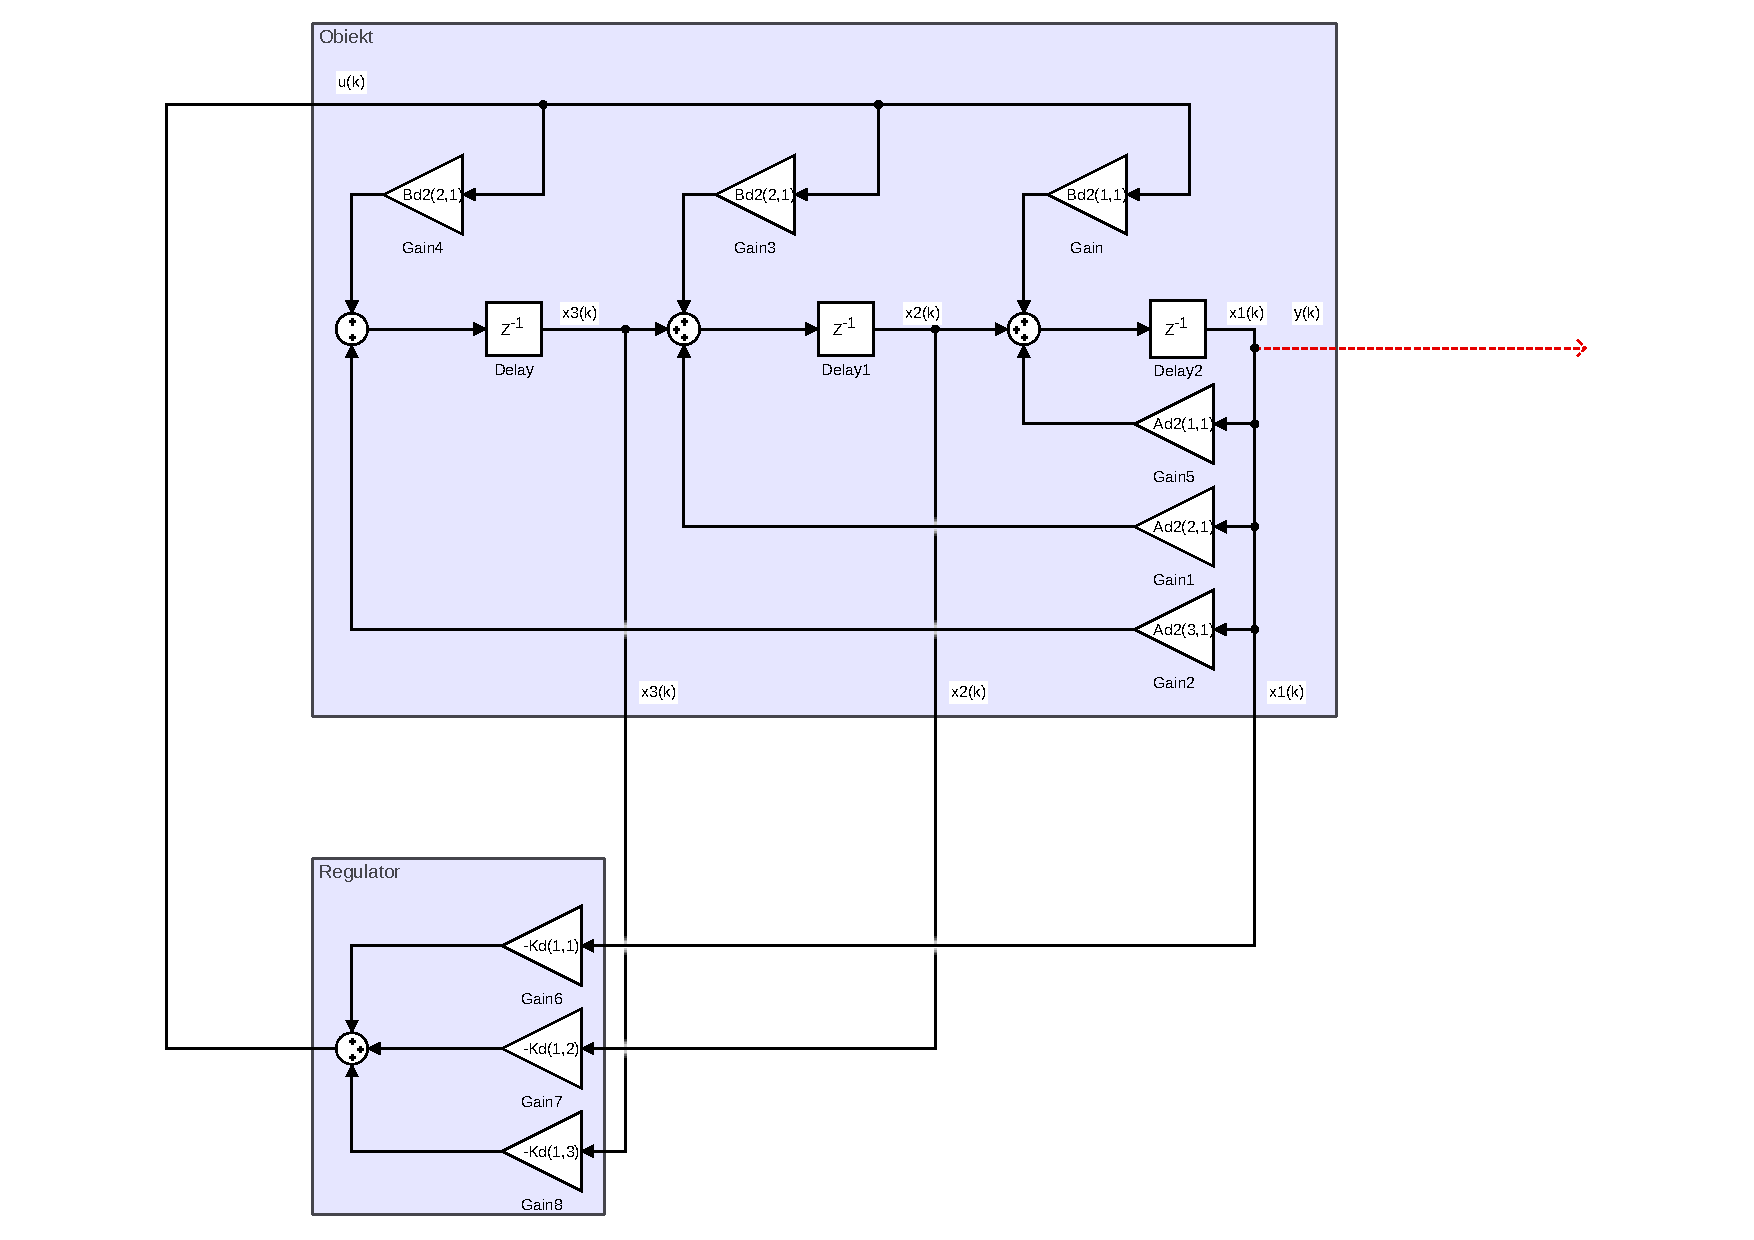
\includegraphics[width=\textwidth]{img/stp5.pdf}
\caption{Struktura układu zamkniętego.}
\end{figure}

\subsection{Trzy takie same bieguny}
Ustawiając trzy bieguny regulatora na tę samą wartość nie jesteśmy w stanie otrzymać stabilnego układu.
Układ jest najwolniej niestabilny w okolicach $z_b \approx 2,5$, co można obliczyć metodą prób i błędów.

\begin{figure}[H]
\centering
 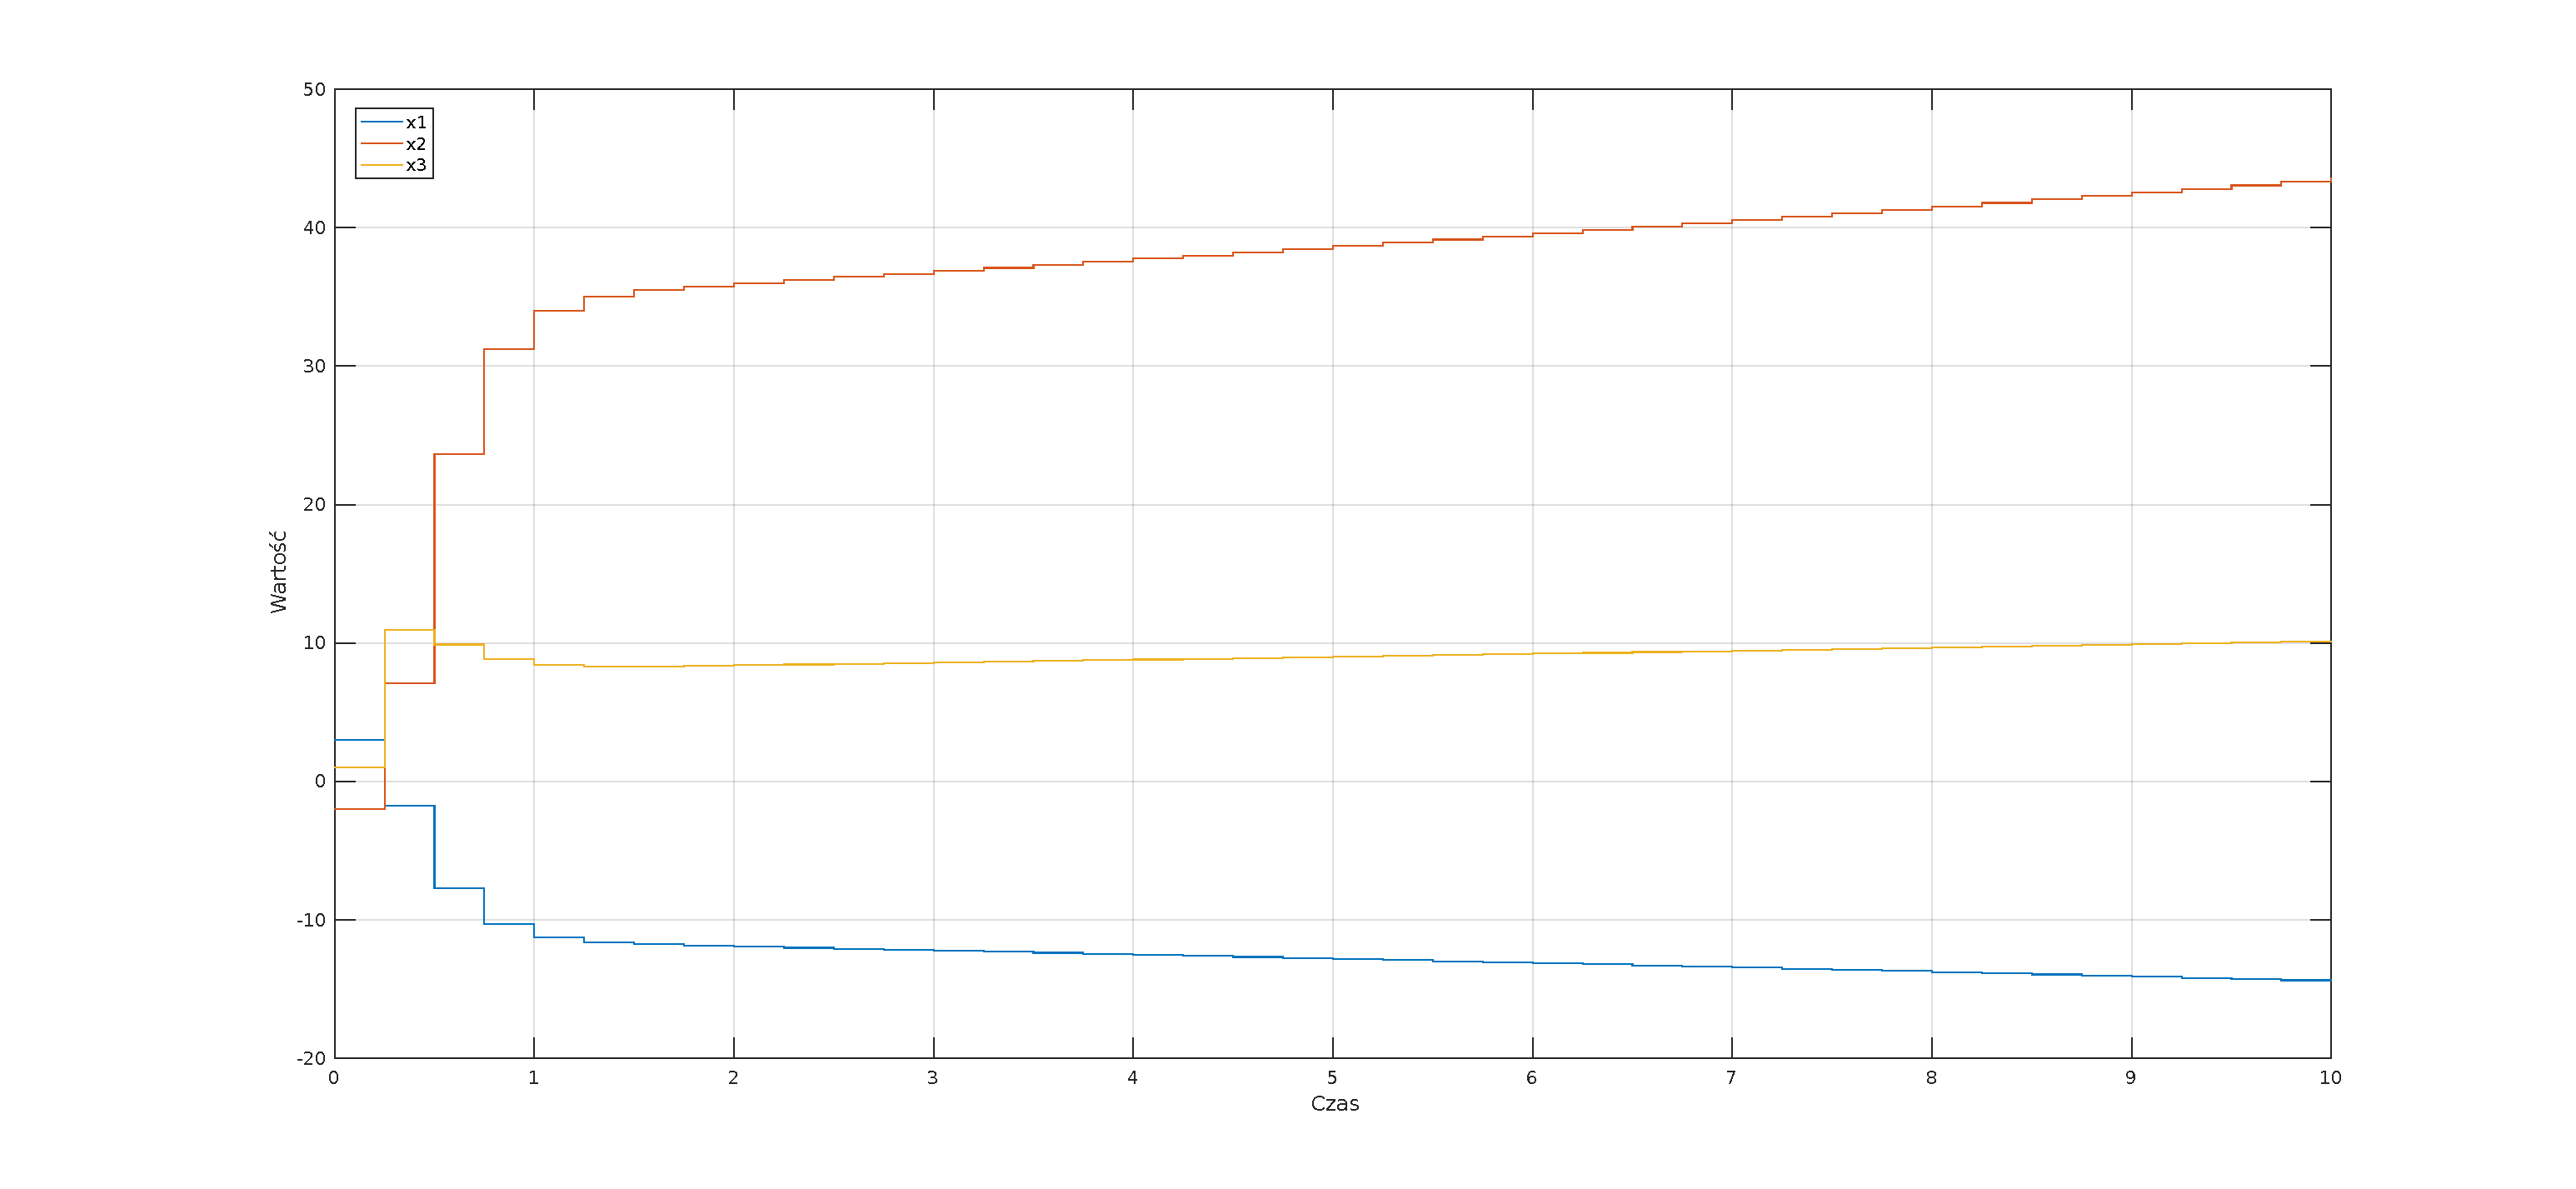
\includegraphics[width=\textwidth]{img/plot5_1.pdf}
\caption{Wartości stanu dla trzech biegunów $\approx 2,5$.}
\end{figure}

